% 正式内容与排版主源。使用 report/tools/build_report.ps1 由XeLaTeX直接生成PDF。
% 中文统一宋体，英文统一Times New Roman；不使用Word主题字体。
\documentclass[UTF8,12pt,a4paper,fontset=none]{ctexart}
\usepackage[left=31.75mm,right=31.75mm,top=25.4mm,bottom=25.4mm,headheight=30pt,headsep=10pt]{geometry}
\usepackage{fontspec}
\setmainfont{Times New Roman}
\setsansfont{Times New Roman}
\setmonofont{Times New Roman}
\setCJKmainfont[AutoFakeBold=2]{SimSun}
\setCJKsansfont[AutoFakeBold=2]{SimSun}
\setCJKmonofont{SimSun}
\usepackage{unicode-math}
\setmathfont{TeX Gyre Termes Math}
\usepackage{graphicx,float,longtable,booktabs,array,calc,amsmath,tikz,fancyhdr,needspace,xurl,hyperref}
\graphicspath{{source/}}
\urlstyle{same}
\hypersetup{hidelinks,pdftitle={基于FPGA的心电边缘分析系统}}
\pagestyle{fancy}\fancyhf{}
\fancyhead[C]{
\includegraphics[height=24pt]{figures/competition_header.png}}
\fancyfoot[C]{\small\thepage}
\renewcommand{\headrulewidth}{0.4pt}
\setcounter{secnumdepth}{0}
\ctexset{section={format=\large\bfseries,beforeskip=14pt,afterskip=7pt},subsection={format=\normalsize\bfseries,beforeskip=10pt,afterskip=5pt},subsubsection={format=\normalsize\bfseries,beforeskip=8pt,afterskip=4pt}}
\setlength{\parindent}{2em}\setlength{\parskip}{2pt}
\linespread{1.15}\setlength{\emergencystretch}{2em}
\setlength{\LTpre}{6pt}\setlength{\LTpost}{6pt}
\tikzset{photolabel/.style={draw=teal!60!black,fill=yellow!4,rounded corners=1pt,inner sep=3pt,font=\fontsize{8.4}{10}\selectfont}}
\begin{document}
\begin{center}{\zihao{-2}\bfseries 基于FPGA的心电边缘分析系统}\par 技术文档\end{center}

\section{摘要}

心电分析需要从连续波形中定位心跳、识别心拍类别，并及时显示结果。本作品以Zynq-7020为核心，构建数据接收、心拍检测、辅助分类和网页显示系统。电脑接收和显示数据，板上ARM处理器完成心拍定位及模型输入整理，FPGA电路承担分类计算。同一硬件设计保留浮点CNN、INT8混合精度CNN和树模型HGB。通过卷积16路输出并行、全连接4路并行及权重存储调整，在不重新训练和更换权重的条件下加快运行。同板60秒合成回放的72个有效心拍中，INT8软件平均每拍7.695ms，FPGA调用0.854ms，加速9.015倍；浮点CNN为4.174倍。调用包含板内数据交换，不含采集、串口、检测和显示。网页关联波形、分类概率及计时，并展示硬件静态资源。

\section{第一部分 作品概述}

\subsection{1.1 功能与特性}

系统接收连续心电数据，也能回放CSV文件，定位心跳、计算RR间隔与心率，再截取单次心拍分类。网页显示波形、类别、概率及耗时，支持浮点或INT8混合精度CNN的整段和边采边测，保留HGB整段分析，并比较同一心拍在ARM与FPGA上的结果和速度。

\subsection{1.2 应用领域}

作品面向生物电信号处理教学、心拍识别算法研究和嵌入式硬件加速实验，可用于观察心电波形、分析心拍节律，以及比较不同模型在处理器和FPGA上的运行效果。

\subsection{1.3 主要技术特点}

ARM处理状态、滤波、心拍检测和模型输入，FPGA利用并行电路加速分类。浮点CNN、INT8混合精度CNN与HGB共存于同一硬件设计，通过同一网页选择。心拍位置对应原波形，计时与分类结果同步保存。

\subsection{1.4 主要性能指标}

{% 无题注的正文表格
\begin{longtable}[]{@{}
  >{\raggedright\arraybackslash}p{(\linewidth - 2\tabcolsep) * \real{0.4301}}
  >{\raggedright\arraybackslash}p{(\linewidth - 2\tabcolsep) * \real{0.5699}}@{}}
\toprule\noalign{}
\begin{minipage}[b]{\linewidth}\raggedright
\textbf{指标}
\end{minipage} & \begin{minipage}[b]{\linewidth}\raggedright
\textbf{测试结果}
\end{minipage} \\
\midrule\noalign{}
\endhead
\bottomrule\noalign{}
\endlastfoot
500Hz心拍检测 & 灵敏度99.8731\%；阳性预测值99.8453\% \\
模型调用加速 & CNN浮点4.174倍；INT8混合精度9.015倍 \\
三核硬件设计 & 工作频率100MHz；各项电路资源占用见3.5节 \\
\end{longtable}
}

\subsection{1.5 主要创新点}

（1）针对树模型与神经网络设计专用电路，在同一芯片保留三种计算路径。（2）通过INT8混合精度量化减少数据位宽，结合卷积16路、全连接4路并行及分层权重存储加速推理。（3）以同拍、同模型和同精度对照验证优化：浮点加速由2.985倍提高到4.174倍，INT8由5.624倍提高到9.015倍。

\subsection{1.6 设计流程}

先完成数据解析、电压换算和显示，再接通检测与分类。将模型核心移入FPGA后，以软件、仿真和板测逐级对照，调整并行结构与权重存储，最后完成持续回放及网页切换。

\section{第二部分 系统组成及功能说明}

\subsection{2.1 整体介绍}

采集模块无线发送数据至电脑，经USB串口转交开发板。ARM检测心跳、整理波形及节律，选定模型分类后，将结果与原始采样位置一同返回网页。

\begin{center}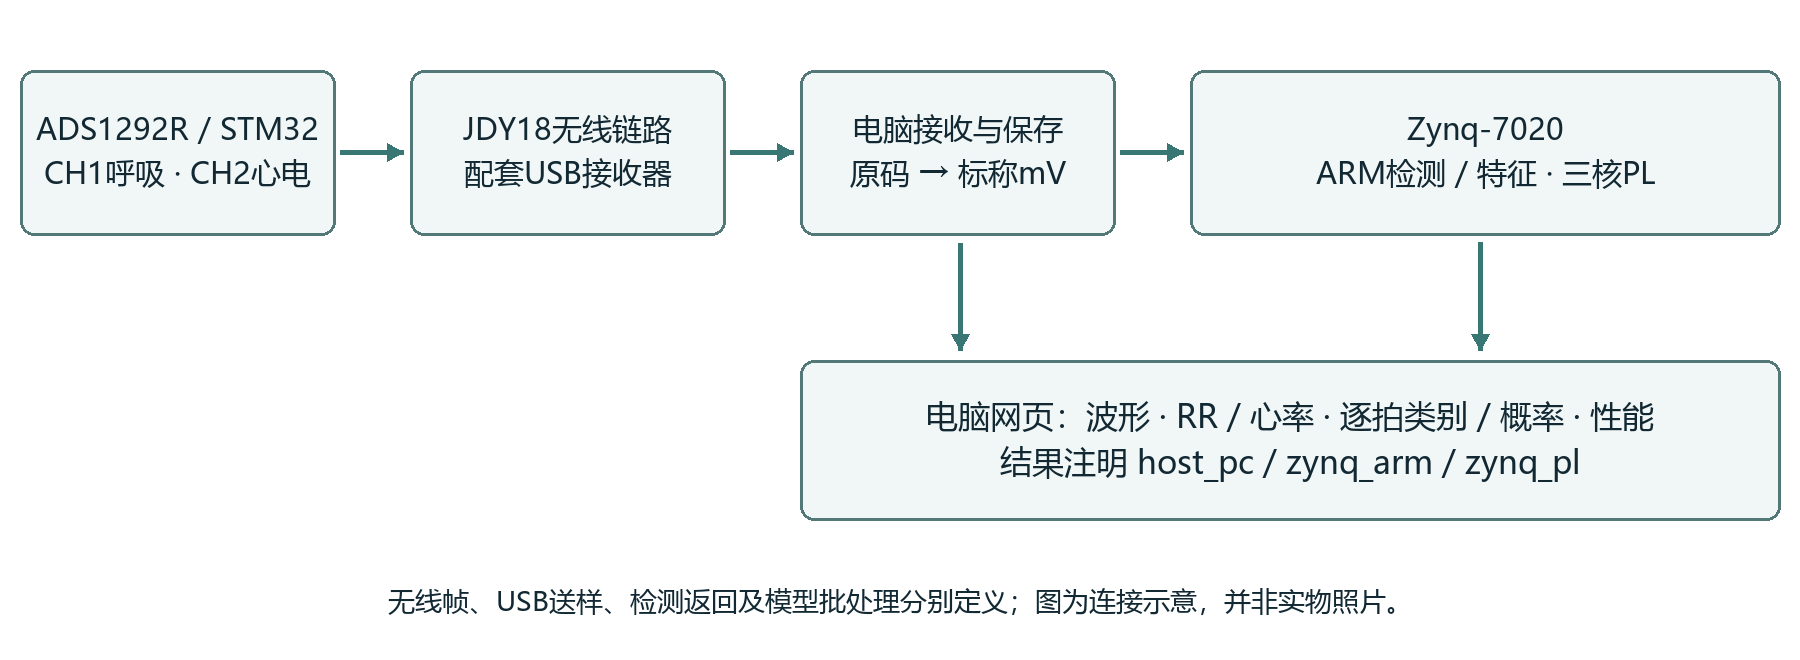
\includegraphics[width=\linewidth]{figures/system.png}\end{center}

\begin{center}\small 系统连接与数据流向\end{center}

\subsection{2.2 硬件系统介绍}

系统采用领航者V2开发板，核心芯片为Zynq-7020。芯片内ARM执行软件和控制任务，可编程逻辑区域（PL）构成专用计算电路。运行数据存放在内存（DDR），板载存储器（QSPI）保留原启动镜像；本文三核设计已在开发板上验证通过。工程使用Vivado/Vitis 2026.1，并用XSim先模拟电路运行、检查结果，开发流程参考文献{[}1{]}{[}2{]}。

采集端用3.7V锂电池供电。ADS1292R将生物电信号转换为原码，STM32经JDY-18蓝牙4.2发送至电脑USB接收器。每包34字节，以AA BB开头，包含CH1呼吸、CH2心电各4点。程序读取每点4字节数据，去除固定偏移，再换算为毫伏。

数字原码减8388608后得到有符号值，再按模块方确认的2.42V参考电压、6倍增益换算为毫伏：

\[v_{\mathrm{mV}} = C_{\mathrm{signed}}\frac{2420}{6 \times 8388607}.\]

换算采用模块方给定的标称参数。手册以\(2^{23}\)为理想分母{[}3{]}，与本式相差约0.000012\%。进入整数检测算法时，每毫伏转换为4096个单位，并按16位范围舍入和限幅；原码与毫伏数据同时保存，便于后续分析。

ARM通过芯片内部接口（AXI-Lite）把输入交给PL，发出启动信号并读回结果。浮点CNN、INT8混合精度CNN、HGB及心拍检测外设集成在同一设计中；当前模型流程的滤波、心拍检测和输入整理由ARM执行。

\subsection{2.3 软件系统介绍}

\subsubsection{2.3.1 分层与通信}

电脑采用网页与后台服务分工的方式（React/TypeScript、FastAPI），提供实时采集、文件回放、记录与导出。网页可选板端模型、CNN精度及整段或边采边测，显示逐拍概率、ARM/FPGA耗时、量化前后类别变化和静态资源；分析期间板上工作灯约2Hz闪烁，结束后熄灭。电脑端HGB另作对照分析。

\begin{center}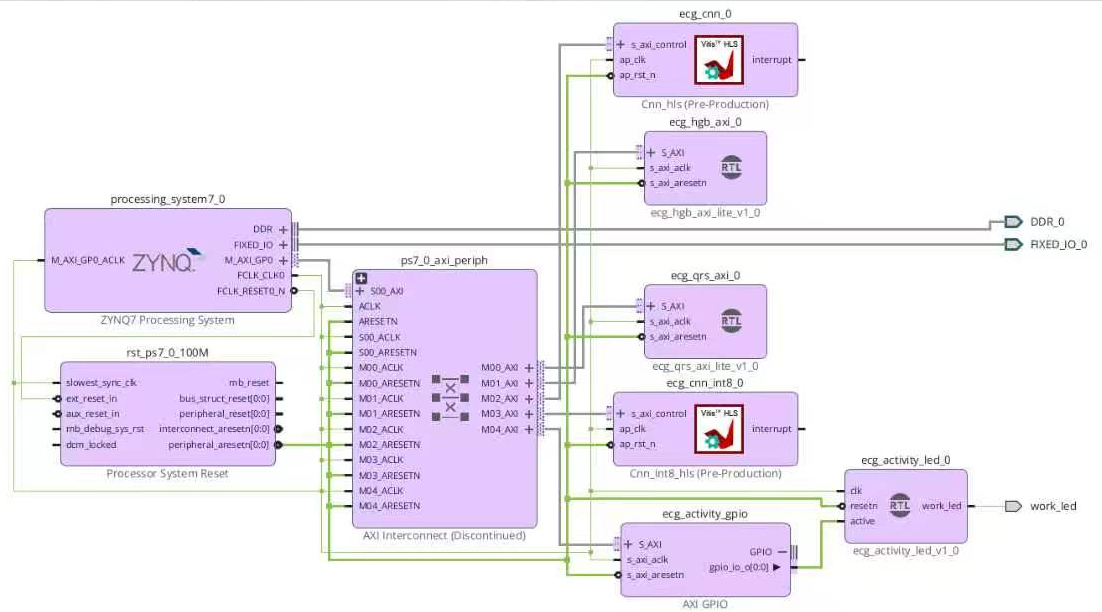
\includegraphics[width=\linewidth]{figures/vivado_block_design.jpg}\end{center}

\begin{center}\small Vivado硬件连接图：ARM经AXI连接浮点CNN、HGB及INT8 CNN\end{center}

采集至电脑解析厂商34字节帧；电脑至开发板传送样本并返回结果。USB串口为115200波特率、8数据位、1停止位，无校验和流控；每块等待板端确认，避免积压。

电脑从0开始为样本编号，根据采样率计算时间，使检测位置和分类结果始终对应同一段波形。连接中断或增益变化时重新建立会话并保存记录。

\subsubsection{2.3.2 滤波、心跳检测与切拍}

先滤波减轻漂移和干扰，再定位心跳（QRS/R峰），由相邻峰间隔（RR）计算心率，最后围绕R峰截取单次心拍（切拍）并分类。

网页保留幅值，纵轴随当前范围调整，不归一化。心电可选原始、0.5Hz高通去基线及节律显示滤波，后者再加40Hz低通和50Hz陷波；呼吸显示用0.05Hz高通和0.8Hz低通。原始记录保留，显示处理独立于板端及模型输入。

检测路径先用1001系数的FIR滤波器抗混叠，按18/25将500Hz转为360Hz，检测后把位置映射回原采样轴。方法参考文献{[}6{]}{[}7{]}的开源实现。

模型路径接收每秒500点的单导联毫伏数据，先用0.5Hz高通减轻波形整体缓慢上下漂移。该滤波只使用当前和过去样本，适合连续处理。下式中x为输入、y为滤波结果，a为系数：

\[a = \frac{500}{500 + 2\pi \times 0.5},\quad y_{0} = 0,\quad y_{n} = a(y_{n - 1} + x_{n} - x_{n - 1}).\]

滤波用64位浮点，连续分块延续状态。R峰前178点与从峰起267点组成心拍，再统一为128点。HGB提取192项形态与节律特征，需要后继RR，最多等待2.5秒；CNN仅用当前心拍与历史。首RR未知或窗口不足时输出UNCLASSIFIED。

\subsubsection{2.3.3 两种模型与软硬件分工}

HGB逐步判断特征条件，CNN通过乘加提取波形特征，因此分别设计专用电路。部署固定为v92 HGB及H27 CNN的第0折权重；该分组用于联调，不按输入患者切换。

CNN分N正常类、S室上性异位、V室性异位和F融合心拍。HGB分N/S/VF，VF合并V、室性逸搏E和F。H27有25,476个参数，结合波形与历史RR分类，由ARM整理输入、PL计算网络。

CNN只保留最近需要的波形和心拍历史，较早的数据用完后循环覆盖。连续收到的数据接着处理，每段只处理一次；收齐单次心拍所需波形后立即分类，尾部波形不足时保留未分类状态。

\subsubsection{2.3.4 硬件加速实现}

树模型需要连续读取特征并判断分支。为减少软件逐条执行的开销，硬件为三个类别设置独立计算路径，共处理64轮、192棵树。节点和参数保存在芯片内部存储中，参数格式转换前后保持各条件判断一致。树模型用整数保存带小数的分数，采用64位Q40格式，其中40位用于小数部分，并按原顺序累加。ARM使用相同规则计算参考分数。

\Needspace{10\baselineskip}
CNN用权重沿波形滑动、加权求和，提取局部特征。高层次综合（HLS）将C/C++代码转换成电路。浮点卷积保持原并行结构，全连接改为同时计算4个输出，分别存放各层权重，减少重复存储。INT8卷积同时计算16个输出，全连接采用4路并行；读取与计算像流水线一样交错，专用算术单元（DSP）承担乘加。下式表示一个卷积输出：

\[z_{o,t} = \sum_i\sum_k x_{i,t+k-p}w_{o,i,k}.\]

ARM写入261项输入，启动电路，再读取4个类别分数。INT8以8位保存权重和激活、32位累计乘加，偏置、残差与缩放仍用浮点数，属于混合精度。权重改存逻辑单元中的分布式存储（LUTRAM），以更多逻辑换取并行能力，使整系统片上存储较上一版减少8块。各路径分别与相同精度的软件对照，不把量化差异算成硬件错误。

\subsection{2.4 复现方法}

工程提供固定权重、源码、构建脚本和运行教程。新版匹配BIT、XSA与ARM程序位于board/cnn\_fast\_20261103，包含可打开布局布线设计的DCP。按教程校验后通过JTAG加载并回放指定数据，核对心拍、结果和耗时；旧QSPI镜像不能与新版三核混用。

\section{第三部分 完成情况及性能参数}

\subsection{3.1 实物与界面}

作品由ADS1292R采集模块、开发板及电脑端组成，自研部分包括FPGA计算逻辑、ARM应用和电脑软件。下图标出了采集端与开发板的主要组成。

\begin{center}\begin{minipage}{\linewidth}\centering
{\small （a）心电采集端与USB无线接收器}\par\vspace{5pt}
\begin{tikzpicture}
\node[anchor=south west,inner sep=0] (photo) at (0,0) {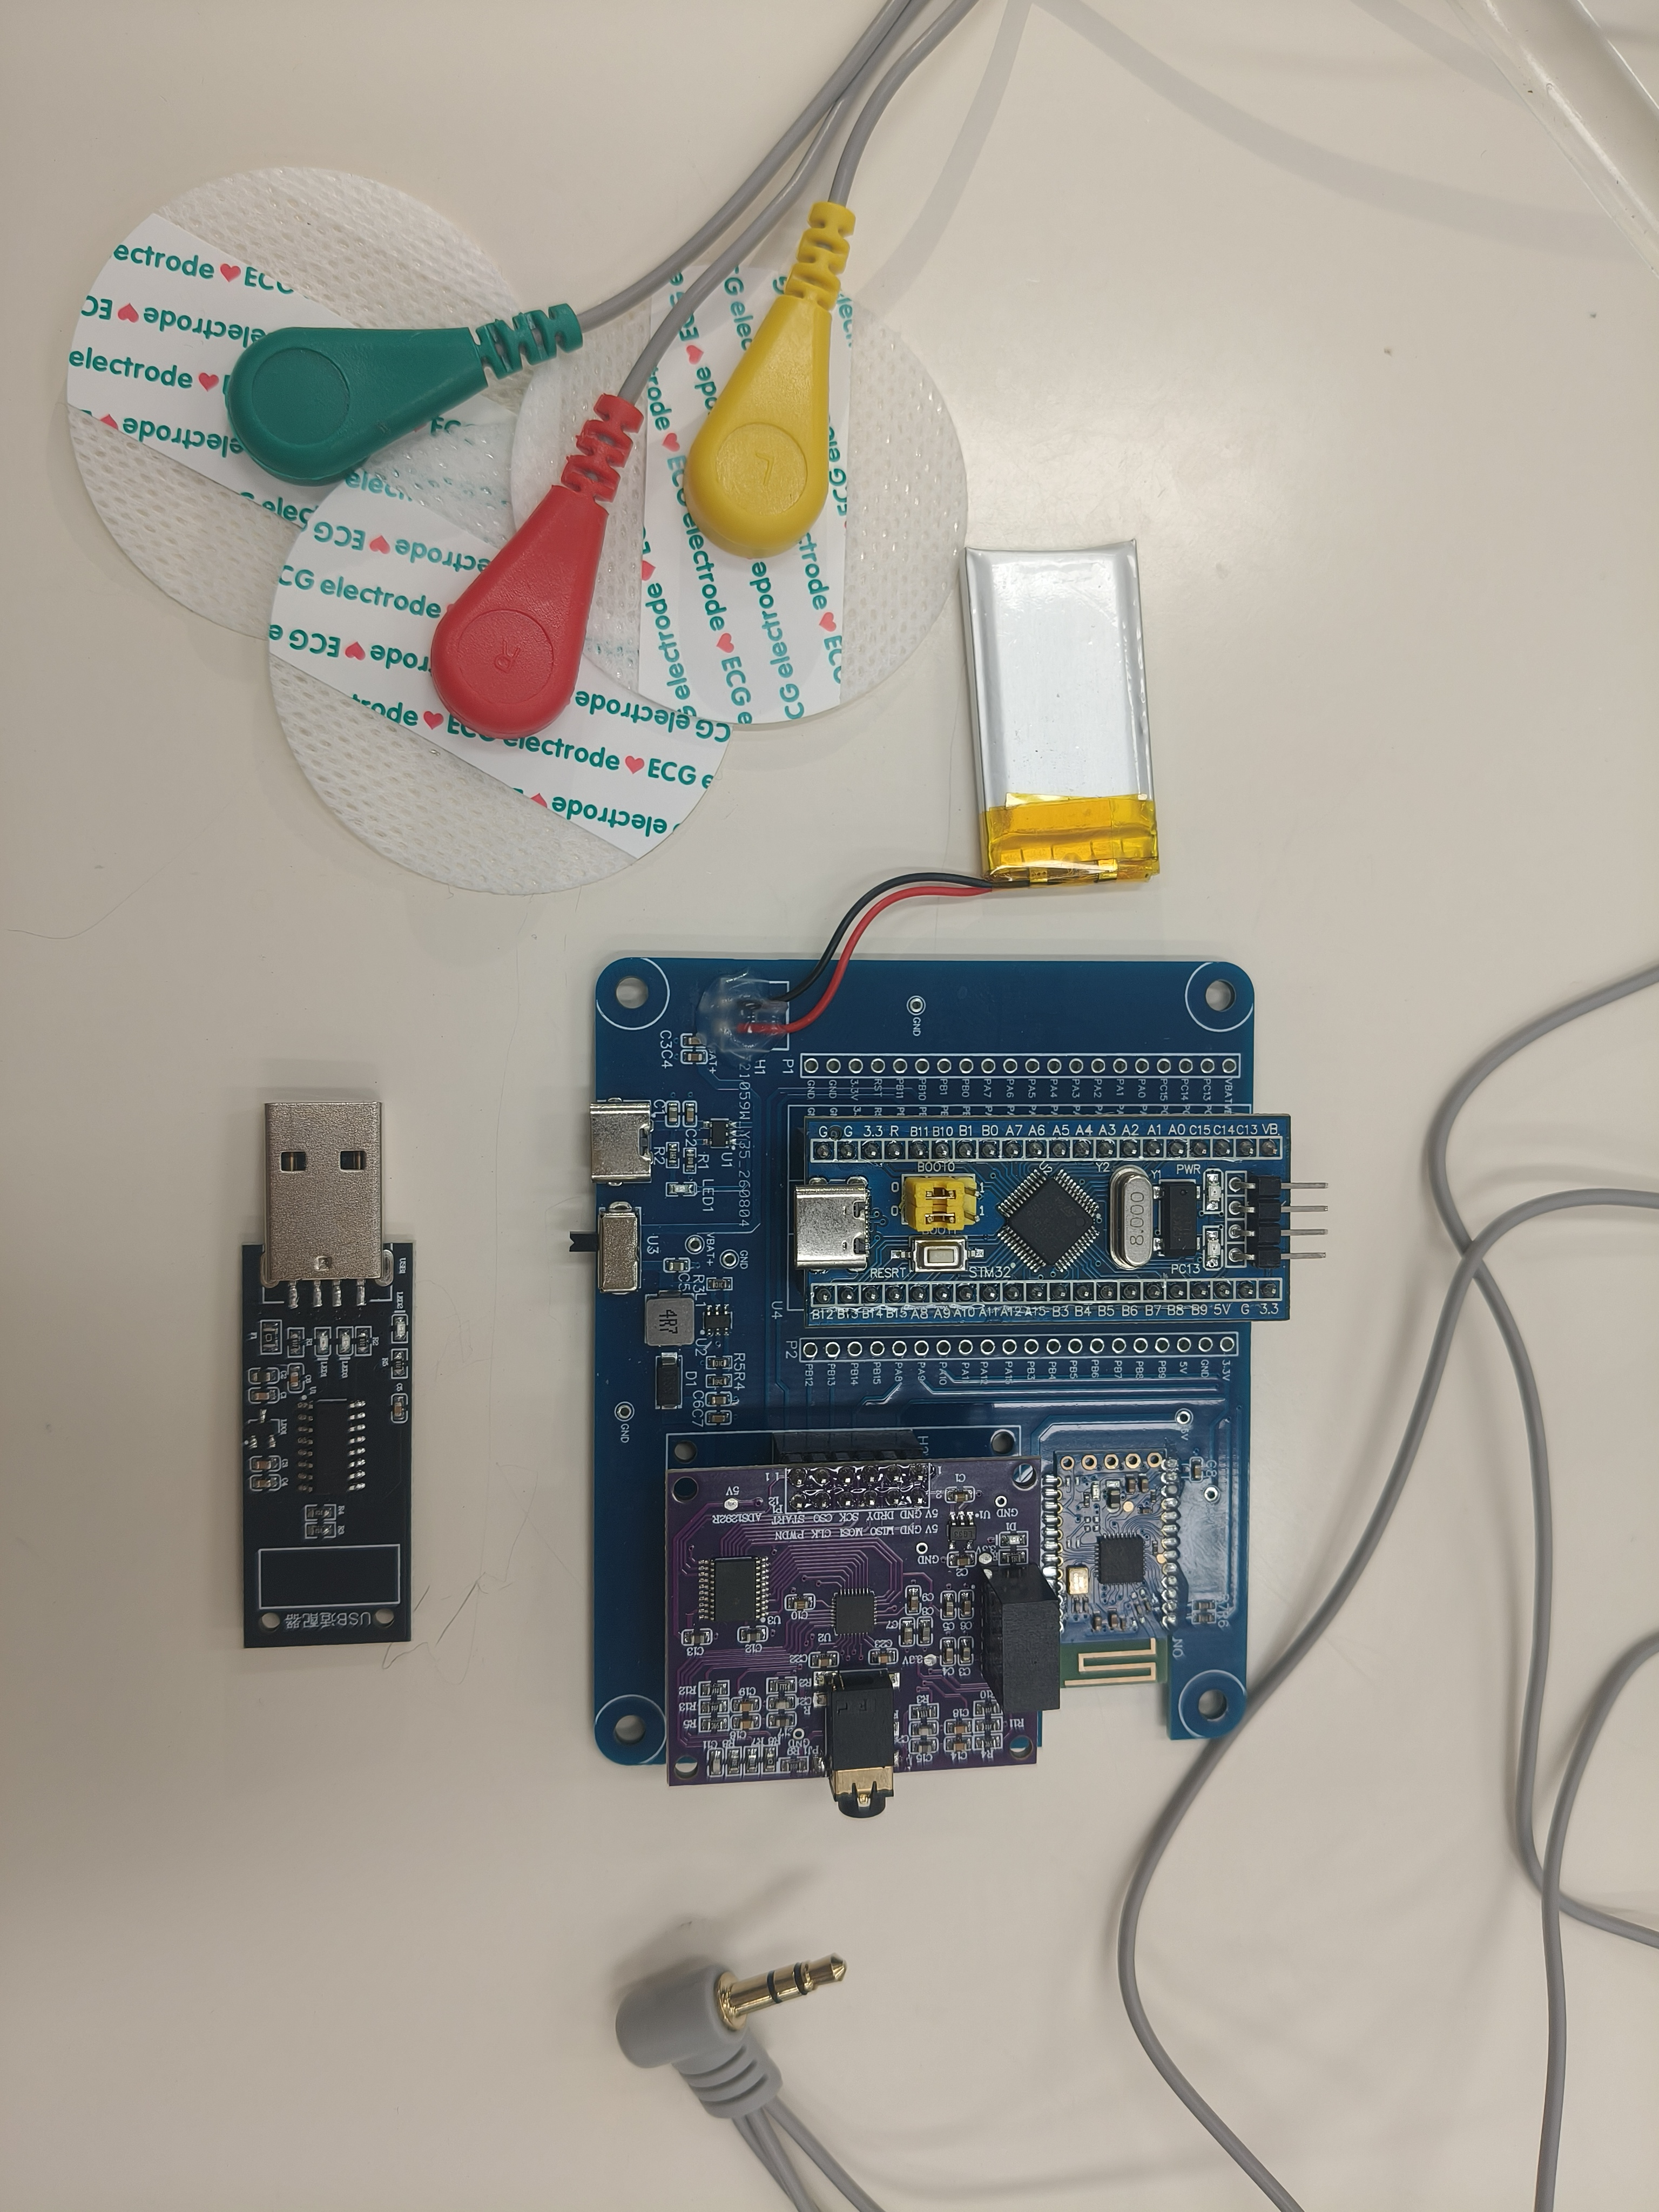
\includegraphics[angle=-90,width=0.92\linewidth]{figures/capture_hardware_original_20261103.jpg}};
\begin{scope}[x={(photo.south east)},y={(photo.north west)}]
\node[photolabel,anchor=north west] (l0) at (0.64,0.96) {电极与导联线};
\draw[orange!85!black,line width=.6pt] (l0) -- (0.81,0.78);
\node[photolabel,anchor=north west] (l1) at (0.62,0.17000000000000004) {3.7V锂电池};
\draw[orange!85!black,line width=.6pt] (l1) -- (0.6799999999999999,0.36);
\node[photolabel,anchor=north west] (l2) at (0.42,0.19999999999999996) {STM32控制板};
\draw[orange!85!black,line width=.6pt] (l2) -- (0.5,0.38);
\node[photolabel,anchor=north west] (l3) at (0.03,0.95) {USB无线接收器};
\draw[orange!85!black,line width=.6pt] (l3) -- (0.36,0.81);
\node[photolabel,anchor=north west] (l4) at (0.03,0.35) {ADS1292R采集板};
\draw[orange!85!black,line width=.6pt] (l4) -- (0.28,0.5);
\node[photolabel,anchor=north west] (l5) at (0.03,0.12) {JDY-18蓝牙模块};
\draw[orange!85!black,line width=.6pt] (l5) -- (0.29000000000000004,0.31999999999999995);
\node[photolabel,anchor=north west] (l6) at (0.02,0.6799999999999999) {电极插头（未接入）};
\draw[orange!85!black,line width=.6pt] (l6) -- (0.09999999999999998,0.54);
\end{scope}
\end{tikzpicture}
\end{minipage}\end{center}

\begin{center}\begin{minipage}{\linewidth}\centering
{\small （b）Zynq开发板与JTAG下载器}\par\vspace{5pt}
\begin{tikzpicture}
\node[anchor=south west,inner sep=0] (photo) at (0,0) {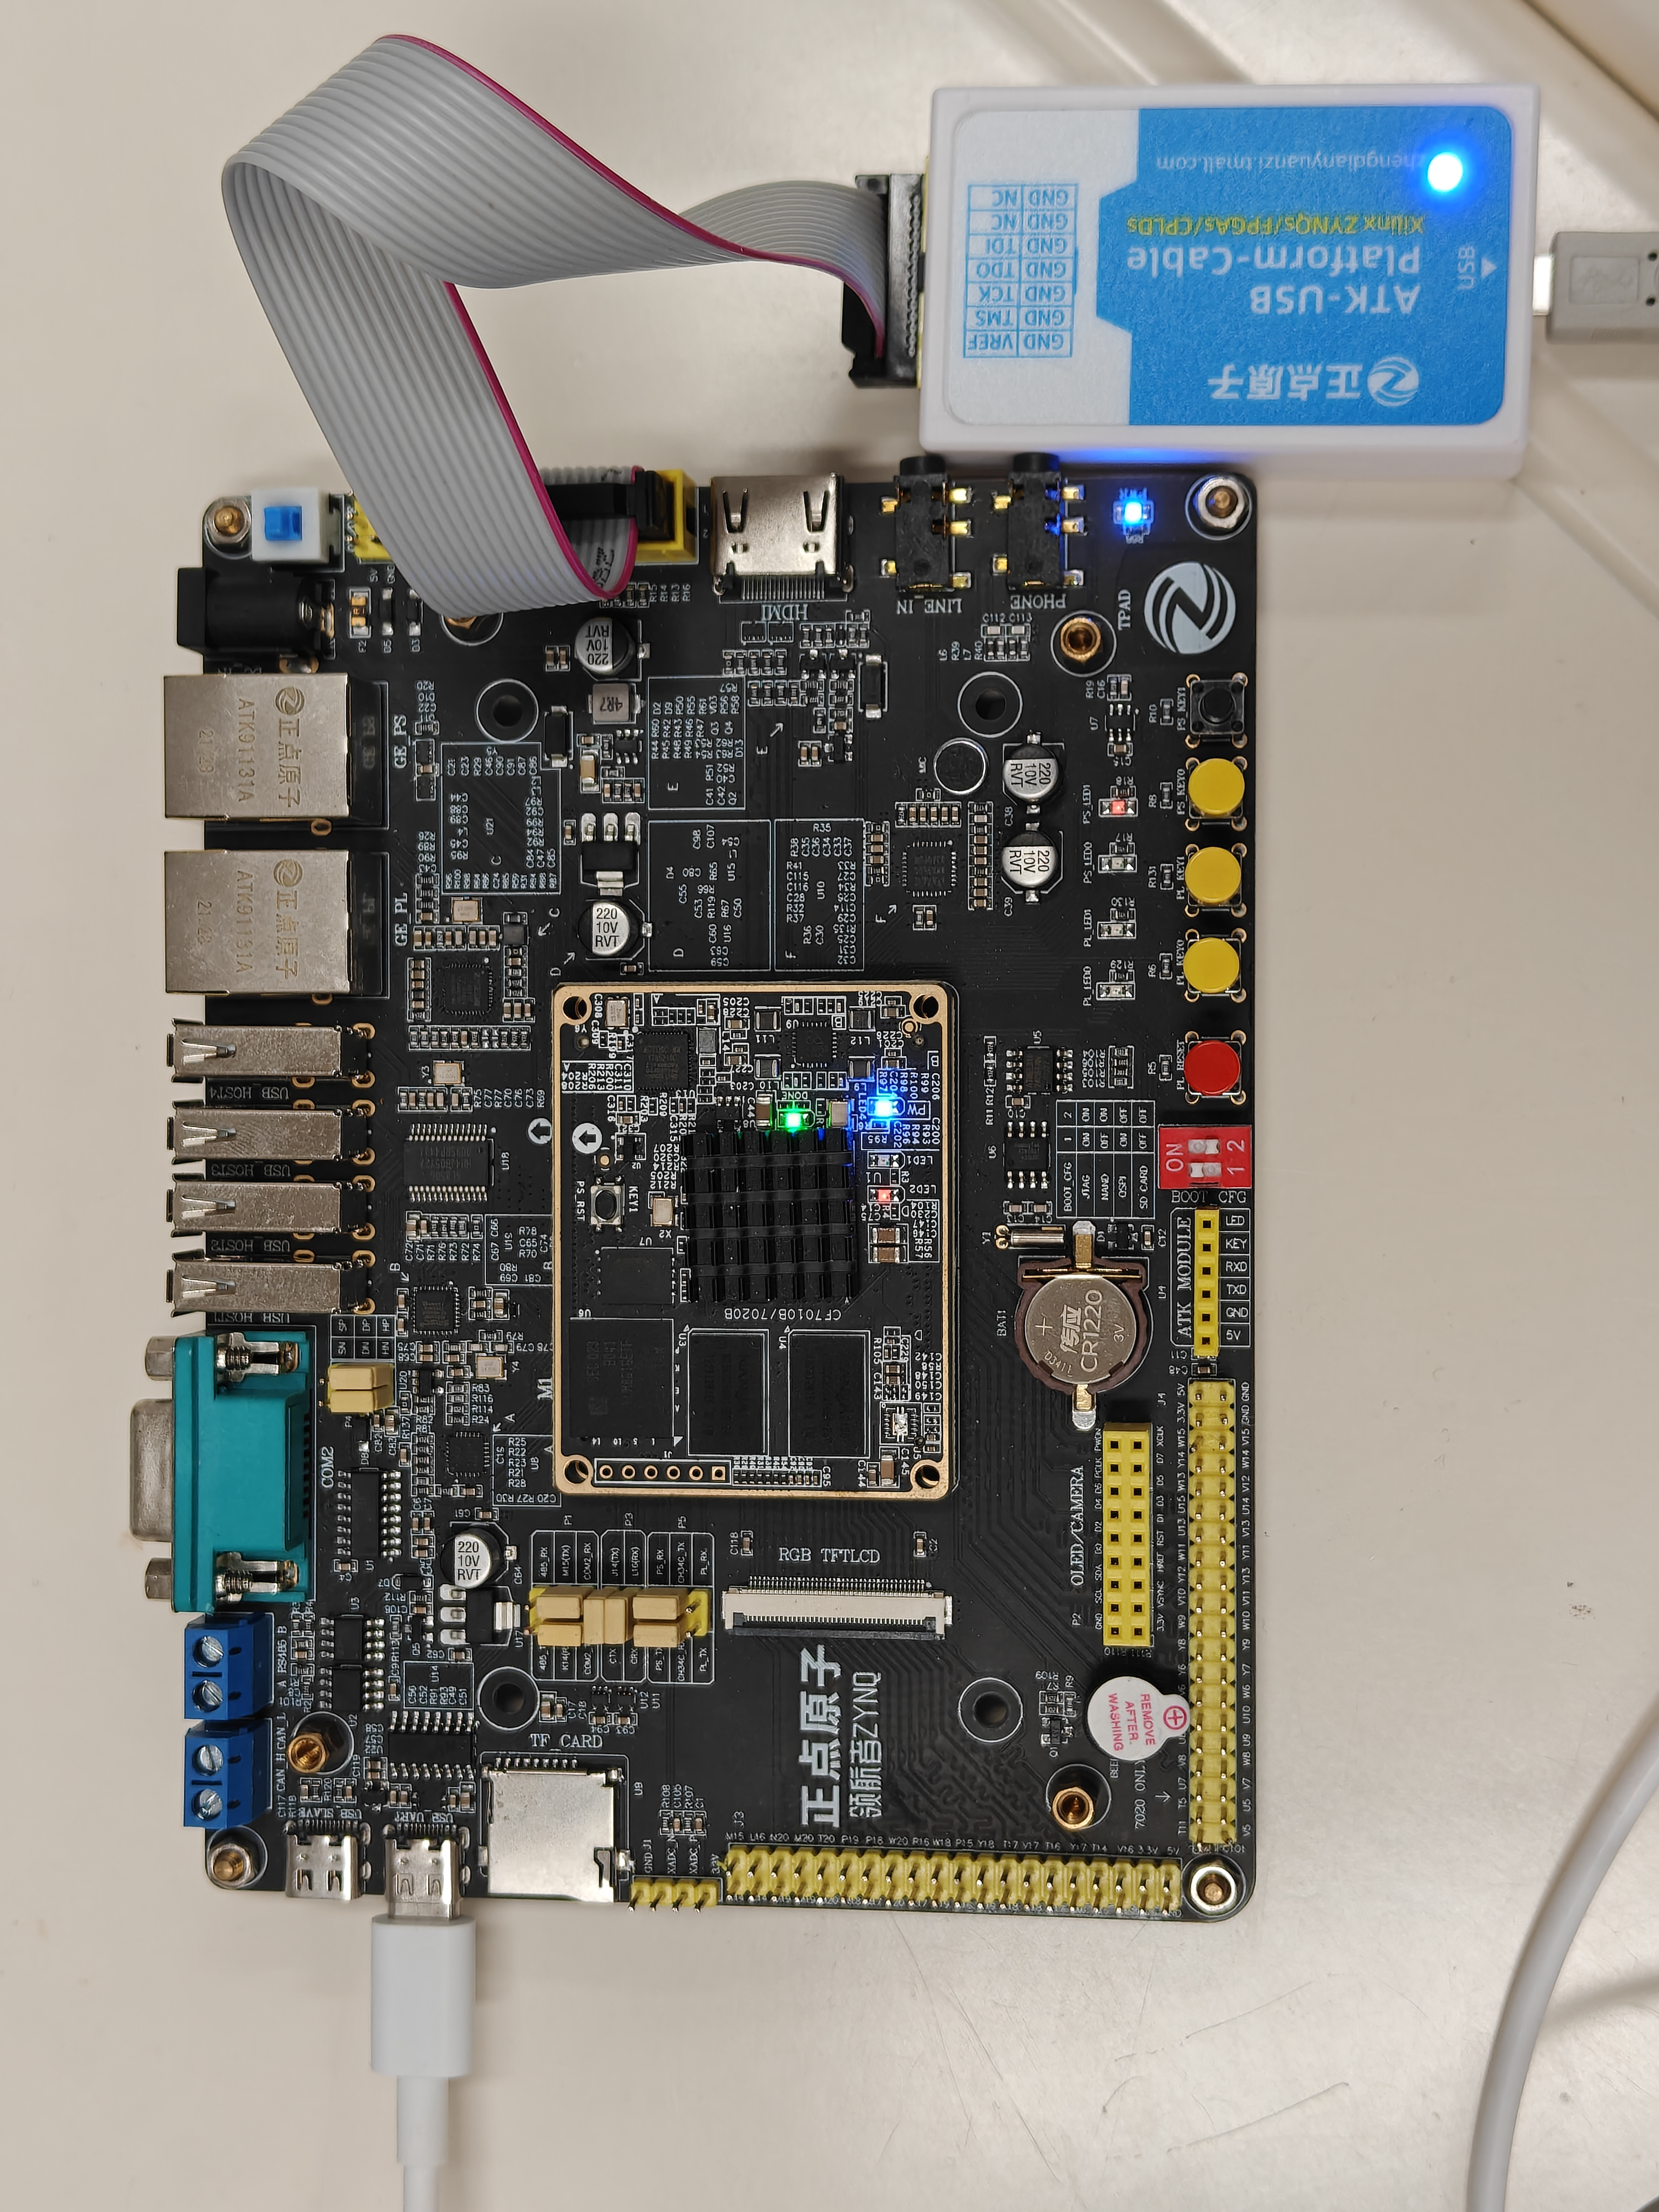
\includegraphics[angle=-90,width=0.92\linewidth]{figures/zynq_hardware_original_20261103.jpg}};
\begin{scope}[x={(photo.south east)},y={(photo.north west)}]
\node[photolabel,anchor=north west] (l0) at (0.61,0.96) {JTAG排线};
\draw[orange!85!black,line width=.6pt] (l0) -- (0.87,0.71);
\node[photolabel,anchor=north west] (l1) at (0.72,0.12) {JTAG下载器};
\draw[orange!85!black,line width=.6pt] (l1) -- (0.88,0.27);
\node[photolabel,anchor=north west] (l2) at (0.7,0.77) {电源开关};
\draw[orange!85!black,line width=.6pt] (l2) -- (0.761,0.829);
\node[photolabel,anchor=north west] (l3) at (0.25,0.69) {Zynq核心板};
\draw[orange!85!black,line width=.6pt] (l3) -- (0.44999999999999996,0.53);
\node[photolabel,anchor=north west] (l4) at (0.4,0.19999999999999996) {模式切换};
\draw[orange!85!black,line width=.6pt] (l4) -- (0.48,0.33499999999999996);
\node[photolabel,anchor=north west] (l5) at (0.02,0.92) {USB\_UART串口};
\draw[orange!85!black,line width=.6pt] (l5) -- (0.14,0.76);
\end{scope}
\end{tikzpicture}
\end{minipage}\end{center}

\subsection{3.2 评价方法与QRS结果}

以42条MIT-BIH记录的专家逐拍标注为参照{[}4{]}{[}9{]}，统计正确检出TP、漏检FN、误检FP、心跳定位及RR误差。灵敏度衡量真实心拍检出比例，阳性预测值衡量输出正确比例。201/202按同一患者处理；下列结果来自开发阶段的回放验证。

{% 无题注的正文表格
\begin{longtable}[]{@{}
  >{\raggedright\arraybackslash}p{(\linewidth - 2\tabcolsep) * \real{0.4301}}
  >{\raggedright\arraybackslash}p{(\linewidth - 2\tabcolsep) * \real{0.5699}}@{}}
\toprule\noalign{}
\begin{minipage}[b]{\linewidth}\raggedright
\textbf{500Hz检测指标}
\end{minipage} & \begin{minipage}[b]{\linewidth}\raggedright
\textbf{测试结果}
\end{minipage} \\
\midrule\noalign{}
\endhead
\bottomrule\noalign{}
\endlastfoot
正确检出/漏检/误检 & 96787 / 123 / 150 \\
真实心拍检出比例/检出结果正确比例 & 99.8731\% / 99.8453\% \\
心跳位置/心跳间隔平均时间误差 & 2.8097ms / 2.8741ms \\
符合既定标准的记录数 & 41/42；105号误检66、漏检10 \\
\end{longtable}
}

使用同一批心电数据比较时，500Hz与360Hz处理结果等效。105号记录的噪声误检是主要改进点；实测波形用于检查数据传输和数值，逐拍准确性使用有专家标注的公开数据评价。

\Needspace{12\baselineskip}
\subsection{3.3 分类质量}

INCART按患者三组轮流训练验证，各组用对应留出模型{[}5{]}。下表为自动检测后分类，包含漏检与额外预测。精确率衡量预测正确比例，召回率衡量该类真实心拍检出比例；F1综合两者，macro-F1对各类等权平均。

{% 无题注的正文表格
\begin{longtable}[]{@{}
  >{\raggedright\arraybackslash}p{(\linewidth - 4\tabcolsep) * \real{0.4201}}
  >{\raggedright\arraybackslash}p{(\linewidth - 4\tabcolsep) * \real{0.3400}}
  >{\raggedright\arraybackslash}p{(\linewidth - 4\tabcolsep) * \real{0.2399}}@{}}
\toprule\noalign{}
\begin{minipage}[b]{\linewidth}\raggedright
\textbf{模型}
\end{minipage} & \begin{minipage}[b]{\linewidth}\raggedright
\textbf{S精确率/召回率}
\end{minipage} & \begin{minipage}[b]{\linewidth}\raggedright
\textbf{汇总指标}
\end{minipage} \\
\midrule\noalign{}
\endhead
\bottomrule\noalign{}
\endlastfoot
HGB三类（0.5Hz高通） & 53.71\% / 81.63\% & macro-F1 86.12\% \\
H27四类 & 50.36\% / 83.69\% & macro-F1 69.10\% \\
H27的F类 & 30.00\% / 16.77\% & F1 21.51\% \\
\end{longtable}
}

以专家标注的全部心拍为分母，自动检测并正确分类的比例为97.70\%。逐类指标显示，S类精确率和F类识别仍有提升空间。两模型的类别划分不同，表中分别列出各自评价结果。

\subsection{3.4 优化前后硬件加速对比}

在同一块Zynq-7020上，对同一H27权重和相同输入，分别运行同精度ARM参考与FPGA。使用500Hz、60秒合成波形，共30000点、73个事件、72个有效心拍；合成输入用于工程计时，不计分类准确率。ARM计时器约333.33MHz，PL为100MHz。比较优化前后的结果，加速比为软件累计耗时除以硬件调用累计耗时：

\[S_{call} = \frac{\sum_{j}^{}T_{ARM,j}}{\sum_{j}^{}T_{PLcall,j}}.\]

{% 无题注的正文表格
\begin{longtable}[]{@{}
  >{\raggedright\arraybackslash}p{(\linewidth - 6\tabcolsep) * \real{0.2000}}
  >{\raggedright\arraybackslash}p{(\linewidth - 6\tabcolsep) * \real{0.2499}}
  >{\raggedright\arraybackslash}p{(\linewidth - 6\tabcolsep) * \real{0.3000}}
  >{\raggedright\arraybackslash}p{(\linewidth - 6\tabcolsep) * \real{0.2501}}@{}}
\toprule\noalign{}
\begin{minipage}[b]{\linewidth}\raggedright
\textbf{模型/精度}
\end{minipage} & \begin{minipage}[b]{\linewidth}\raggedright
\textbf{ARM（ms/拍）}
\end{minipage} & \begin{minipage}[b]{\linewidth}\raggedright
\textbf{FPGA调用（ms/拍）}
\end{minipage} & \begin{minipage}[b]{\linewidth}\raggedright
\textbf{加速倍率}
\end{minipage} \\
\midrule\noalign{}
\endhead
\bottomrule\noalign{}
\endlastfoot
FP32优化前 & 8.247736 & 2.763185 & 2.985 \\
FP32优化后 & 8.247995 & 1.976009 & 4.174 \\
INT8优化前 & 7.694013 & 1.368123 & 5.624 \\
INT8优化后 & 7.694567 & 0.853556 & 9.015 \\
\end{longtable}
}

同精度优化后，浮点调用耗时降低28.49\%，INT8降低37.61\%，分类结果均与各自优化前一致。同批心拍的优化INT8调用比优化浮点快2.315倍，收益来自量化、并行及存储的共同调整。硬件调用含写入、计算等待和结果读取，不含无线、USB串口、滤波、检测、切拍、概率转换或网页；9.015倍仅指模型调用加速。

230组固定向量中，优化INT8、原INT8与独立整数参考逐位一致；12组电路联合仿真最大分数误差为0。72拍板测同精度结果不一致为0；INT8与浮点有5拍类别不同，不能写量化没有精度损失。原浮点12组仿真最大分数误差为\(2.861\times10^{-6}\)，HGB保留原492组仿真及160组特征实板对照证据。

\Needspace{12\baselineskip}
\subsection{3.5 资源占用与持续处理}

{% 布局布线后三阶段资源对比
\begin{longtable}{@{}>{\raggedright\arraybackslash}p{0.30\linewidth}>{\raggedleft\arraybackslash}p{0.14\linewidth}>{\raggedleft\arraybackslash}p{0.14\linewidth}>{\raggedleft\arraybackslash}p{0.17\linewidth}>{\raggedleft\arraybackslash}p{0.13\linewidth}@{}}
\toprule
\textbf{阶段} & \textbf{LUT} & \textbf{FF} & \textbf{BRAM} & \textbf{DSP} \\
\midrule
\endhead
\bottomrule
\endlastfoot
原三核 & 23386 & 18426 & 121 & 92 \\
浮点优化后 & 24147 & 19789 & 130.5 & 89 \\
INT8优化后 & 28626 & 20458 & 122.5 & 105 \\
最终使用率 & 53.81\% & 19.23\% & 87.50\% & 47.73\% \\
\end{longtable}
}

表中为布局布线后三核整系统静态资源，非实时负载。LUT为逻辑、FF为状态存储、BRAM为片上存储、DSP为算术单元；器件容量依次为53200、106400、140和220。BRAM按36Kb等效块统计。浮点优化阶段同时增加工作灯，BRAM升至130.5块；调整INT8并行结构和权重存储后降至122.5块，以更多LUT和DSP换速度。100MHz建立/保持余量分别为+0.102/+0.036ns。

500Hz节拍流式回放同一60秒合成输入，72个有效拍的INT8软件平均7.700ms、硬件调用0.854ms，加速9.020倍，同精度不一致为0。整段INT8累计软件554.009ms、硬件调用61.456ms。5148点已采集CSV的四种CNN模式各按CNN→HGB→CNN切换，共12会话且轮间不复位；8份CNN输出经独立复算通过。新版三核已通过板上回放验证。

\section{第四部分 总结}

\subsection{4.1 可扩展之处}

后续可从识别效果与使用体验两方面改进：增加不同人群和噪声条件的数据，重点提高S类、F类识别，并用新患者数据检验效果，减少反复选型带来的偏差{[}8{]}；优化INT8量化，减小与浮点分类结果的差异。工程方面可继续压缩片上存储、完善输出时序约束，并开展长时间无线运行、功耗及采集到显示的整体延迟测试。

\subsection{4.2 心得体会与AI协作}

实现过程使我们理解了数据、算法与硬件的联系：原码需换算物理单位，模型需适应存储和并行电路，结果需对应原波形。AI参与检索、编码与测试组织，成员负责确定目标、核实硬件和审查修改。

\subsubsection{原始提示、对应回答与纠错摘录}

2026年10月25日，用户：``你这个交接写的有问题，是别人用这个工程，不是我。''AI：``我会把交接改成面向接手者：说明他拿到工程后怎么启动、需要准备什么、哪些结果可以复用，去掉依赖你这台电脑和本次聊天的表述。''

2026年10月26日，用户：``原始数据是经过ADC放大的，不是真实电压值''。AI：``上次说`直接接收能用'省略了换算这一步，容易让你误解。''后续依据实际34字节固件及模块方参数，明确了原码到标称电压的换算方法。

以上为封存会话的删节摘录，原文日期、位置与校验索引保存在本地附件。

\subsubsection{人工采纳依据与个人补充}

两次纠错推动了交接说明和电压换算的修正。成员按真实环境、波形位置和数值对照审查AI建议，保留原始回答与修正依据。

从交接换行改变文件、输出错位、下载路径报错、并行化增加存储和计时口径混淆中，提炼文件校验、参考比对、下载诊断、资源时序核查、公平计时五项技能。各项列出适用、操作与失效条件，脚本只需Python标准库。在独立含空格目录及另一工作路径下，25项行为测试通过；计时工具从已有72拍记录复算9.020倍。提示词模板为事后提炼，与原始对话分开，不代替板测。

\section{第五部分 参考文献}

{[}1{]} 全国大学生嵌入式芯片与系统设计竞赛. FPGA创新设计赛道选题指南 AMD{[}S{]}. 2026: 自主选题3.3.3---3.3.5.

{[}2{]} AMD. Vitis统一软件平台文档 嵌入式软件开发 UG1400{[}EB/OL{]}. 2026.1版, 2026{[}2026-11-03{]}. \url{https://docs.amd.com/r/zh-CN/ug1400-vitis-embedded}.

{[}3{]} Texas Instruments. 用于生物电势测量的ADS129x低功耗、双通道、24位模拟前端{[}Z{]}. ZHCS146C（英文版SBAS502C）, 2020年4月修订: 8.3.4及8.3.8节.

{[}4{]} Moody G, Mark R. MIT-BIH Arrhythmia Database, version 1.0.0{[}DB/OL{]}. PhysioNet, 2005. DOI:10.13026/C2F305.

{[}5{]} Yakushenko E. St Petersburg INCART 12-lead Arrhythmia Database, version 1.0.0{[}DB/OL{]}. PhysioNet, 2008. DOI:10.13026/C2V88N.

{[}6{]} MIT-LCP. WFDB-Python qrs.py{[}CP/OL{]}. v4.3.1{[}2026-11-03{]}. \url{https://github.com/MIT-LCP/wfdb-python/blob/v4.3.1/wfdb/processing/qrs.py}.

{[}7{]} Makowski D, Pham T, Lau Z J, et al. NeuroKit2: A Python toolbox for neurophysiological signal processing{[}J{]}. Behavior Research Methods, 2021, 53(4):1689--1696. DOI:10.3758/s13428-020-01516-y.

{[}8{]} Cawley G C, Talbot N L C. On Over-fitting in Model Selection and Subsequent Selection Bias in Performance Evaluation{[}J{]}. Journal of Machine Learning Research, 2010, 11(70):2079--2107.

{[}9{]} Pollard T, Moody B E, Lehman L H, et al. PhysioNet as a global platform for biomedical research{[}J{]}. Nature Health, 2026, 1(8):792-795. DOI:10.1038/s44360-026-00096-z.

\end{document}
